\chapter{Formalising ML Problem Settings}



\section{Machine Learning from the Mathematical Perspective}

What is machine learning?


\begin{tcolorbox}[title=Professor, colback=yellow!20!white, colframe=orange!35!black, sharp corners]
    Machine learning is the study of algorithms which automatically perform a task by processing an example dataset.
\end{tcolorbox}


\begin{tcolorbox}[title=ChatGPT, colback=purple!10!white, colframe=violet!40!black, sharp corners]
    Machine learning is a computational approach that allows systems to automatically learn and improve from experience without being explicitly programmed.
\end{tcolorbox}

The professor himself much prefers his definition, which focuses on the word \textbf{algorithms}, \textbf{task}, and \textbf{dataset}.\\

The issue with the GPT definition is that the word `computational' is too broad and vague, and the notion of `learn' and `improving from experience' is too colloqiually used in the actual nature of machine learning.

\section{Datasets}
Data is the keystone of machine learning, used to infer and learn good models. We denote the input or feature space as $x \in \mathbb{R}^n$ and outputs as $y \in \mathbb{R}^m$.

There are several ways we can look at data:

\begin{figure}
    \centering
    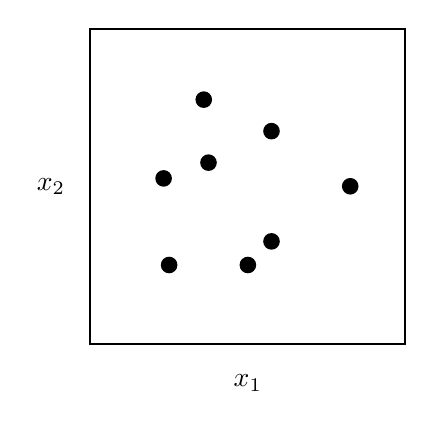
\begin{tikzpicture}
        % Draw the outer square
        \draw[thick, black] (0,0) rectangle (4,4);

        % Draw the black points
        \fill[black] (1.44,3.1) circle (3pt);
        \fill[black] (1.5,2.3) circle (3pt);
        \fill[black] (0.93,2.1) circle (3pt);
        \fill[black] (2.3,2.7) circle (3pt);
        \fill[black] (3.3,2) circle (3pt);
        \fill[black] (2.3,1.3) circle (3pt);
        \fill[black] (2,1) circle (3pt);
        \fill[black] (1,1) circle (3pt);
        % Labels for the axes
        \node at (2,-0.5) {$x_1$};
        \node at (-0.5,2) {$x_2$};
    \end{tikzpicture}
    % \caption{Simplified example for $f^\theta$}
    % \label{fig:1_classification}
\end{figure}
% A simplified example for $f^\theta$ is shown in Figure \ref{fig:1_classification}. Ideally, we want a separator that separates the input space into $m$ distinct regions according to observed data.


\subsection{Set Perspective}
\begin{itemize}
    \item Data is viewed as a collection of $N$ 2-tuples: $\{(x^{(i)}, y^{(i)})\}_{i=1}^{N}$, where each input-output pair is part of the dataset.
    \item This perspective is order/permutation invariant, focusing on the set of samples rather than the order in which they appear.
    \item The size of the set measures the sample complexity.
    \item Sets are often useful for reasoning about feature/label spaces in an abstract way.
    \item Example of dataset representation:


          \[
              \{ (\bm{x}^{(i)})_{i=1}^{N} \}
          \]This represents a dataset consisting of a collection of $N$ input vectors $\bm{x}^{(i)}$. Each $\bm{x}^{(i)}$ is a feature vector or a sample, without any corresponding labels or outputs. This kind of dataset is typically used in unsupervised learning, where we only have inputs and are not concerned with outputs (e.g., clustering or dimensionality reduction).


          \[
              \{ (\bm{x}^{(i)}, \bm{y}^{(i)})_{i=1}^{N} \}
          \]This represents a set of $N$ input-output pairs, where $\bm{x}^{(i)}$ is the input feature vector and $\bm{y}^{(i)}$ is the corresponding label or output. This is the standard representation for datasets in supervised learning, where the goal is to learn a function that maps inputs to outputs (e.g., regression or classification tasks).


          \[
              \{ (\bm{s}^{(i)}, \bm{a}^{(i)}, \bm{s}^{(i+1)})_{i=1}^{N} \}
          \]This set represents a sequence of $N$ tuples, where $\bm{s}^{(i)}$ is the state at time step $i$, $\bm{a}^{(i)}$ is the action taken in that state, and $\bm{s}^{(i+1)}$ is the resulting next state. This kind of dataset is commonly used in reinforcement learning (RL), where the goal is to learn a policy that dictates which actions to take in various states to maximize a reward signal over time.



\end{itemize}

\subsection{Probability Perspective}
\begin{itemize}
    \item Data is viewed as samples where each sample is a 2-tuple $(\bm{x}^{(i)}, \bm{y}^{(i)})$ drawn from a joint distribution $P(\mb{X},\mb{Y})$, where the relationship between input $\mb{X}$ and output $\mb{Y}$ is of primary interest.
    \item We are interested in the probability of an output given we have observed a particular input: $P(\mb{Y}=\bm{y} | \mb{X}=\bm{y})$.
    \item This perspective is fundamental in probabilistic machine learning and provides tools for modelling uncertainty and reasoning about observations.
    \item Common assumptions like i.i.d. (independent and identically distributed) are often applied:
          \[
              P(x_1, x_2, \dots, x_k) = P(x_1) \cdot P(x_2) \dots P(x_k)
          \]
    \item Example of dataset representation with probabilistic modeling:

          \[
              \bm{x} \sim P(\mathbf{X})
          \]
          This represents an input vector $\bm{x}$ sampled from a probability distribution $P(\mathbf{X})$. In this case, $\mathbf{X}$ refers to the input space, and each input $\bm{x}$ is drawn according to its distribution.


          \[
              (\bm{x}, \bm{y}) \sim P(\mathbf{X}, \mathbf{Y})
          \]
          This represents an input-output pair $(\bm{x}, \bm{y})$ sampled from the joint distribution $P(\mathbf{X}, \mathbf{Y})$, where $\mathbf{X}$ refers to the input space, and $\mathbf{Y}$ refers to the output space. The goal here is to model the relationship between inputs $\bm{x}$ and corresponding outputs $\bm{y}$, as is typical in supervised learning.

          \[
              \bm{s}^{(i+1)} \sim P(\bm{s}^{(i+1)} \mid \bm{s}^{(i)}, \bm{a}^{(i)})
          \]
          This represents the next state $\bm{s}^{(i+1)}$ sampled from the conditional probability distribution given the current state $\bm{s}^{(i)}$ and action $\bm{a}^{(i)}$. This kind of representation is typical in reinforcement learning (RL), where we model transitions between states based on actions taken by the agent.

\end{itemize}


\subsection{Linear Algebra/Statistics Perspective}
\begin{itemize}
    \item A bit misleading to call it a `linear algebra perspective' since it's used here in almost al of statistics.
    \item Data is treated as vectors and matrices. An input is a vector $\bm{x} \in \mathbb{R}^{n \times 1}$x, collected into a matrix $X \in \mathbb{R}^{m \times n}$, with $m$ samples and $n$ features.
          \[
              \bm{x} = \begin{bmatrix}
                  x_1 \\ x_2 \\ \vdots \\ x_n
              \end{bmatrix} \quad X = \begin{bmatrix}
                  \bm{x}^{(1)\top} \\ \bm{x}^{(2)\top} \\ \vdots \\ \bm{x}^{(m)\top}
              \end{bmatrix} = \begin{bmatrix}
                  x_1^{(1)} & x_2^{(1)} & \dots  & x_n^{(1)} \\
                  x_1^{(2)} & x_2^{(2)} & \dots  & x_n^{(2)} \\
                  \vdots    & \vdots    & \ddots & \vdots    \\
                  x_1^{(m)} & x_2^{(m)} & \dots  & x_n^{(m)}
              \end{bmatrix}
          \]
    \item Each row of the matrix represents a data sample (input vector), and columns correspond to features (called explanatory variables in statistics). The matrix is often referred to as the \textit{design matrix}.
    \item This perspective allows the application of linear algebra tools to study properties like rank, invertibility, and dimensionality reduction.
    \item The labels (response variables) $y \in \mathbb{R}^{m \times 1}$ are collected into a vector:
          \[
              x = \begin{pmatrix}
                  x_1^{(1)} & x_2^{(1)} & \dots  & x_n^{(1)} \\
                  x_1^{(2)} & x_2^{(2)} & \dots  & x_n^{(2)} \\
                  \vdots    & \vdots    & \ddots & \vdots    \\
                  x_1^{(m)} & x_2^{(m)} & \dots  & x_n^{(m)}
              \end{pmatrix}, \quad \mathbf{y} = \begin{pmatrix}
                  y_1 \\ y_2 \\ \vdots \\ y_m
              \end{pmatrix}
          \]
\end{itemize}

\section{Types of Learning Tasks}

There are several types of learning tasks that can be broadly classified into the following categories:

\subsection{Supervised Learning}
In supervised learning, we train models using input-output pairs, where the correct output (label) is known. The goal is to learn a mapping from inputs to outputs. For example, given a dataset of customer transaction data and their purchase categories, the task is to predict future purchases based on transaction history. \bigskip

There are also two types of supervised learning tasks:
\begin{enumerate}
    \item \textbf{Regression:} The output variable is continuous, such as predicting house prices based on square footage.
    \item \textbf{Classification:} The output variable is discrete (categorical), such as classifying emails as spam or not spam.
\end{enumerate}

\subsection{Unsupervised Learning}
Unsupervised learning involves learning from data without labeled outputs. The objective is to discover hidden patterns or groupings in the data. An example is clustering news articles into different topics based on the text content, without prior knowledge of the categories. \bigskip

Unsupervised learning comes in convenient if we have huge amounts of data without labels, and we want to extract meaningful insights from it without having to manually label each data point (which is almost often done manually and can be expensive).



\subsection{Generative Learning}
Generative learning aims to model the underlying data distribution and generate new data samples that resemble the training data. For instance, a generative model could be trained on music tracks and then used to generate new compositions that sound like the originals. This can be in a supervised or unsupervised setting.

\subsection{Algorithms}
Back to the definition of machine learning:
\begin{tcolorbox}[title=Professor, colback=yellow!20!white, colframe=orange!35!black, sharp corners]
    Machine learning is the study of algorithms which automatically perform a task by processing an example dataset.
\end{tcolorbox}

\textbf{Algorithms} are not the same as \textbf{models}. Instead, models are assumed/inferred and algorithms returned learned models.

Without getting into many technicalities, it is difficult to convey meaningful algorithmic difference, thus this section will be answered throughout the course.

\section{The Linear Model}

Choosing a model in machine learning is deciding how we think inputs and outputs can be releated. The most basic linear model assumes that the output is a weighted linear combination of the input features. Weights are represented by vector $\bm{w}$, and the model is represented as:

\begin{equation}
    \hat{y} = \bm{w}^\top \bm{x}  := \sum_{i=1}^{n} w_i x_i
\end{equation}

The above model would be learned by an \textbf{algorithm} from the dataset, where the algorithm decides what the weights should be. The model is then used to make predictions on new data points. \bigskip

This is a dot product between the weight vector $\bm{w}$ and the input feature vector $\bm{x}$. Keen readers will note out that this only model lines that cross through the origin, however there will be methods to extend this model to lines that do not cross through the origin. \bigskip

One such way would be to normalize the data so it can always be represented by a line through the origin.

\section{Data Preprocessing: Normalising the Data}
Given the limitations of the linear model in the previous section, data normalisation allows us to transform the data so that it can be modelled by a line through the origin.

\subsection{Naive Method}
Assuming no noise and outlier, normalisation can be naively done (s) by the following steps:

\begin{itemize}
    \item Pick an arbitrary feature-label pair in the dataset, $(\bm{x}^{(i)}, y^{(i)})$.
    \item Subtract $\bm{x}^{(i)}$ from all input features and $y^{(i)}$ from all target labels.
    \item The data has been transformed.
\end{itemize}
\intuitb{Example for 1D \ensuremath{x} and 1D \ensuremath{y}}{
    \begin{itemize}
        \item The points can be described by the relationship $y = mx + b$ where $b$ is the bias.
        \item The bias is preventing us from modelling the data with the relationship $y = mx$.
        \item We choose an arbitrary point in the dataset to be subtracted from all points
        \item We can choose any point because all points contain the bias component.
        \item After subtracting, all bias components are removed, and the data can be modelled by a line through the origin.
    \end{itemize}
}

\begin{figure}[h]
    \centering
    \begin{subfigure}{0.5\linewidth}
        \centering
        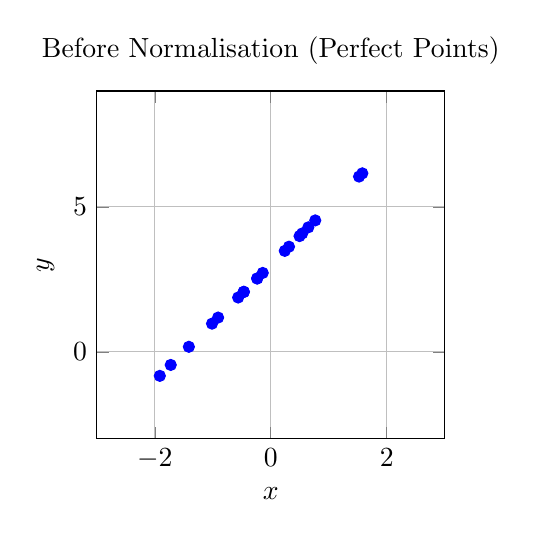
\begin{tikzpicture}
            \begin{axis}[
                    title={Before Normalisation (Perfect Points)},
                    xlabel={$x$}, ylabel={$y$},
                    width=6cm, height=6cm,
                    grid=major,
                    xmin=-3, xmax=3,
                    ymin=-3, ymax=9,
                    scatter/classes={a={mark=o,draw=blue}},
                    scatter, only marks,
                ]
                \addplot[scatter,only marks, mark=*,blue] coordinates {
                        (0.4967141530112327, 3.9934283060224653) (-0.13826430117118466, 2.723471397657631) (0.6476885381006925, 4.295377076201385) (1.5230298564080254, 6.046059712816051) (-0.23415337472333597, 2.531693250553328) (-0.23413695694918055, 2.531726086101639) (1.5792128155073915, 6.158425631014783) (0.7674347291529088, 4.534869458305818) (-0.4694743859349521, 2.0610512281300957) (0.5425600435859647, 4.085120087171929) (-0.46341769281246226, 2.0731646143750755) (-0.46572975357025687, 2.068540492859486) (0.24196227156603412, 3.4839245431320682) (-1.913280244657798, -0.8265604893155958) (-1.7249178325130328, -0.44983566502606553) (-0.5622875292409727, 1.8754249415180546) (-1.0128311203344238, 0.9743377593311524) (0.3142473325952739, 3.628494665190548) (-0.9080240755212109, 1.1839518489575782) (-1.4123037013352915, 0.17539259732941703) };
            \end{axis}
        \end{tikzpicture}
        \caption{Before Normalisation (Perfect Points)}
    \end{subfigure}%
    \hfill
    \begin{subfigure}{0.5\linewidth}
        \centering
        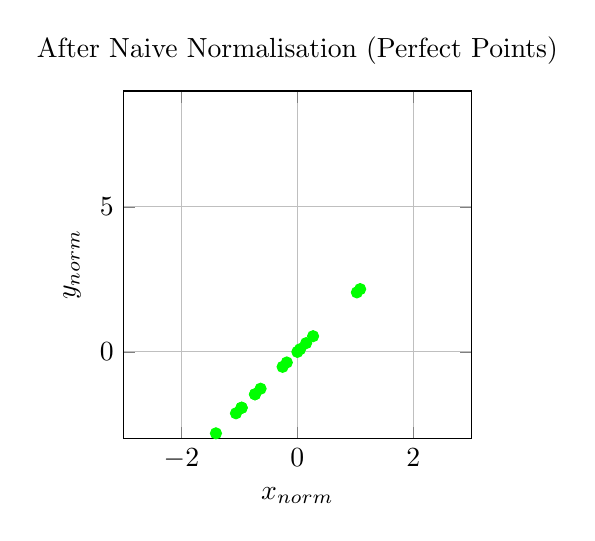
\begin{tikzpicture}
            \begin{axis}[
                    title={After Naive Normalisation (Perfect Points)},
                    xlabel={$x_{norm}$}, ylabel={$y_{norm}$},
                    width=6cm, height=6cm,
                    grid=major,
                    xmin=-3, xmax=3,
                    ymin=-3, ymax=9,
                    scatter/classes={a={mark=o,draw=green}},
                    scatter, only marks,
                ]
                \addplot[scatter,only marks, mark=*,green] coordinates {
                        (0.0, 0.0) (-0.6349784541824173, -1.2699569083648343) (0.15097438508945982, 0.3019487701789193) (1.0263157033967927, 2.052631384006586) (-0.7308675277345686, -1.4617350554691377) (-0.7308511099604132, -1.4617022199208263) (1.0824986624961588, 2.165230539992318) (0.2707205761416761, 0.5414411522833521) (-0.9661885389461848, -1.9323770778923695) (0.045845890574731984, 0.09169178114946397) (-0.9601318458236949, -1.924332605095516) (-0.9624439065814896, -1.928956726611105) (-0.25475188144519856, -0.515471676338523) (-2.4099943976690303, -4.8199887953380605) (-2.221631985524265, -4.44326397104853) (-1.0590016822522053, -2.118003364504411) (-1.5095452733456565, -3.0190905466913136) (-0.1824668204159588, -0.3650668628319176) (-1.4047382285324437, -2.809476457064887) (-1.9090178543465242, -3.818035708693048) };
            \end{axis}
        \end{tikzpicture}
        \caption{After Naive Normalisation}
    \end{subfigure}
    \caption{Comparison of before and after naive normalisation.}
\end{figure}


We almost never use this method, as it is not robust to noise and outliers. We will discuss a more robust method in the next section.

\subsection{Z-Score Normalisation}
There is always be noise and outliers in the data. So instead of picking an arbitrary point to subtract from all points, we can use the mean of the input features and target values and subtract them from all points. \bigskip

We also divide by the standard deviation to scale the data. This is called \textbf{standardisation} or \textbf{z-score normalisation}. \bigskip


We begin by calculating the mean of the input features and the target values:

\begin{equation}
    \bm{x}^{\mu} = \frac{1}{N} \sum_{i=1}^{N} \bm{x}^{(i)} \quad\quad y^{\mu} = \frac{1}{N} \sum_{i=1}^{N} y^{(i)}
\end{equation}

Next, we compute the standard deviation for both the input features and target values:

\begin{equation}
    \bm{x}^{\sigma} = \sqrt{\frac{1}{N} \sum_{i=1}^{N} \left( \bm{x}^{(i)} - \bm{x}^{\mu} \right)^2}\quad\quad y^{\sigma} = \sqrt{\frac{1}{N} \sum_{i=1}^{N} \left( y^{(i)} - y^{\mu} \right)^2}
\end{equation}

Once we have computed the mean and standard deviation, we can normalise the data by subtracting the mean and dividing by the standard deviation. This centres the data around the origin and scales it:

\begin{equation}
    \tilde{\bm{x}}^{(i)} = \frac{\bm{x}^{(i)} - \bm{x}^{\mu}}{\bm{x}^{\sigma}}\quad\quad\tilde{y}^{(i)} = \frac{y^{(i)} - y^{\mu}}{y^{\sigma}}
\end{equation}

The normalised data, $\tilde{\bm{x}}^{(i)}$ and $\tilde{y}^{(i)}$, can now be used in the linear model, which will allow it to handle cases where the data does not necessarily pass through the origin. \bigskip

By centring and scaling the data, the linear model becomes more robust, especially when dealing with non-centred data. This is because the impact of outliers are reduced when subtracted by the mean of the points and scaled down by the standard deviation.

\sn{Division by standard deviation}{
    The curriculum notes only mention subtraction of the mean, and do not include the division by the standard deviation. Subtraction of the mean has a centring effect and an absolute reduction of outliers, however it is mostly the scaling by the standard deviation that reduces the (relative) impact of outliers.
}

\begin{figure}[h!]
    \centering
    % Subfigure for "Before Normalisation"
    \begin{subfigure}{0.5\linewidth}
        \centering
        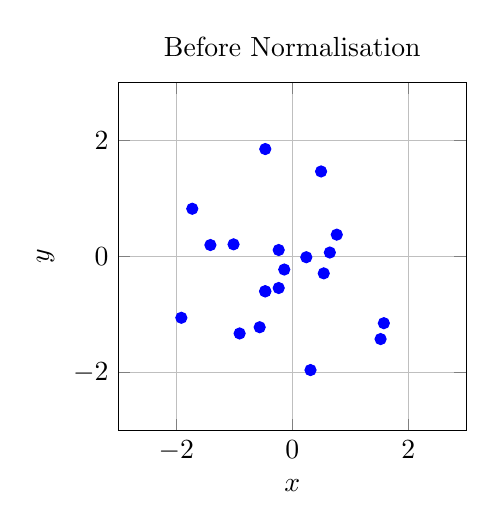
\begin{tikzpicture}
            \begin{axis}[
                    title={Before Normalisation},
                    xlabel={$x$}, ylabel={$y$},
                    width=6cm, height=6cm,
                    grid=major,
                    xmin=-3, xmax=3,
                    ymin=-3, ymax=3,
                    scatter/classes={a={mark=o,draw=blue}},
                    scatter, only marks,
                ]
                \addplot[scatter,only marks, mark=*,blue] coordinates {
                        (0.4967141530112327, 1.465648768921554) (-0.13826430117118466, -0.22577630048653566) (0.6476885381006925, 0.06752820468792384) (1.5230298564080254, -1.4247481862134568) (-0.23415337472333597, -0.5443827245251827) (-0.23413695694918055, 0.11092258970986608) (1.5792128155073915, -1.1509935774223028) (0.7674347291529088, 0.37569801834567196) (-0.4694743859349521, -0.600638689918805) (0.5425600435859647, -0.2916937497932768) (-0.46341769281246226, -0.6017066122293969) (-0.46572975357025687, 1.8522781845089378) (0.24196227156603412, -0.013497224737933921) (-1.913280244657798, -1.0577109289559004) (-1.7249178325130328, 0.822544912103189) (-0.5622875292409727, -1.2208436499710222) (-1.0128311203344238, 0.2088635950047554) (0.3142473325952739, -1.9596701238797756) (-0.9080240755212109, -1.3281860488984305) (-1.4123037013352915, 0.19686123586912352) };
            \end{axis}
        \end{tikzpicture}
        \caption{Before Normalisation}
    \end{subfigure}%
    \hfill
    % Subfigure for "After Normalisation"
    \begin{subfigure}{0.5\linewidth}
        \centering
        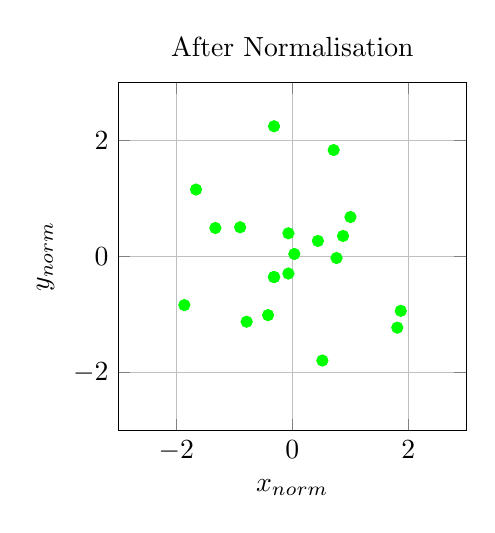
\begin{tikzpicture}
            \begin{axis}[
                    title={After Normalisation},
                    xlabel={$x_{norm}$}, ylabel={$y_{norm}$},
                    width=6cm, height=6cm,
                    grid=major,
                    xmin=-3, xmax=3,
                    ymin=-3, ymax=3,
                    scatter/classes={a={mark=o,draw=green}},
                    scatter, only marks,
                ]
                \addplot[scatter,only marks, mark=*,green] coordinates {
                        (0.713902389388804, 1.8352660925069428) (0.03530357555875783, 0.04260481887952363) (0.8752480822475349, 0.3534643640739835) (1.8107216820007925, -1.228128662954733) (-0.06717267563237075, -0.295071031049124) (-0.06715513002591085, 0.3994560162782024) (1.8707641750195225, -0.9379891264580541) (1.0032203349648776, 0.6800789452558444) (-0.31865925446928695, -0.3546940627728778) (0.7628977005809812, -0.027257961781428666) (-0.312186491902963, -0.3558259030205282) (-0.3146573815487583, 2.245036287536186) (0.44165012093621053, 0.26758935125914035) (-1.8616485270607728, -0.8391232680575755) (-1.6603464063200226, 1.1536707916626914) (-0.4178482718925614, -1.012019908124294) (-0.8993423202038642, 0.5032590463194493) (0.5189008628298603, -1.7950670744823134) (-0.7873354704866504, -1.1257870297401338) (-1.3262569939841797, 0.4905383146690989) };
            \end{axis}
        \end{tikzpicture}
        \caption{After Normalisation}
    \end{subfigure}
    \caption{Example of a 1-dimension feature $x$ and 1-dimensional output $y$. Comparison of points before and after normalisation.}
\end{figure}




% \begin{marginfigure}
%     \centering
%     \begin{tikzpicture}
%         \begin{axis}[
%                 view={0}{90},
%                 axis on top,
%                 enlargelimits=false,
%                 colormap/viridis,
%                 xlabel={$x_1$},
%                 ylabel={$x_2$},
%                 % colorbar,
%                 samples=50, % Adjusting the sample size
%                 domain=-5:5,
%                 width=2in,
%                 height=2in
%             ]

%             % First contour group
%             \addplot3[
%                 contour gnuplot={
%                         levels={0.25, 0.4, 0.55, 0.65, 0.79, 1, 1.25, 1.5}
%                     }
%             ]
%             {exp(-((x)^2 + (1.4*y)^2))};

%             % Second contour group
%             \addplot3[
%                 contour gnuplot={
%                         levels={0.25, 0.4, 0.55, 0.65, 0.79, 1, 1.25, 1.5}
%                     }
%             ]
%             {exp(-((2*x+2)^2 + (y+2)^2))};

%         \end{axis}
%     \end{tikzpicture}
%     \caption{Viewing the dataset as an empirical distribution}
%     \label{fig:1_distribution}
% \end{marginfigure}




% \sn{On The Rigour of A Random Variable}{
%     For the beginning of this module, a random variable $X$ is considered to be a function from a sample space $\Omega$ to the unit interval $[0, 1]$. However, in Lectures 6 and 7, we use the full definition of a random variable, which is a measurable function from a sample probability space $(\Omega)$ to a measurable space $(E, \varepsilon)$, involving the concept of $\sigma$-algebras and measure spaces. \bigskip

%     When the sample space is a continuous space, the function $p$ is a \textbf{probability density function} (PDF). When the sample space is a discrete space, the function $p$ is a \textbf{probability mass function} (PMF).
% }


% \marginnote[-60pt]{We will introduce measure theory later.}





% \section{Brief Probability Theory Review}


% \subsection{Dealing with Data (Single-Feature)}

% In Machine Learning (ML), we often deal with large datasets from which we aim to extract meaningful insights. It is useful to model these data points as random variables:
% \[
%     \{x_1, x_2, \ldots, x_N\}
% \]


% \noindent We typically model these samples as random variables:

% \[
%     \{x_1 \sim X_1, x_2 \sim X_2, \ldots, x_N \sim X_N\}
% \]

% \subsection{Vectors of Random Variables}

% When dealing with joint random variables, we often represent them as vectors:

% \[
%     \mathbf{X} = (X_1, X_2, X_3) \quad \text{with joint distribution} \quad p_{X_1, X_2, X_3}(x_1, x_2, x_3)
% \]

% \noindent For a vector of random variables \(\mathbf{X}\) in \( \mathbb{R}^3 \), the joint probability density function is denoted as:

% \[
%     p_{\mathbf{X}}(\mathbf{x}) \quad \text{where} \quad \mathbf{X} \in \mathbb{R}^3
% \]
% \noindent
% If these are input observations, they are often referred to as "feature vectors."

% \subsection{Distinct Random Variables}

% We model samples as distinct random variables \sidenote[][-20pt]{\textbf{Why should we model these as distinct random variables? Aren't they all the same thing?} \smallskip

%     \noindent Despite being identically distributed, distinct random variables allow for capturing dependencies and interactions between different samples.
% }:\bigskip

% \[
%     \{x_1 \sim X_1, x_2 \sim X_2, \ldots, x_N \sim X_N\}
% \]


% \section{Statistical Modelling as Curve Fitting}

% Machine learning and statistics have significant overlap, and so most concepts studied in this module can be cast as statistical modelling. Consider our random variables:

% \begin{equation}
%     \{x_1 \sim X_1, x_2 \sim X_2, \ldots, x_N \sim X_N\}
% \end{equation}

% \noindent These random variables can be modelled to fit certain curves that represent the underlying data distribution.

% \subsection{Assumption about the Model}

% To proceed with statistical modelling, we make an assumption about the form of the model:

% \begin{equation}
%     P_X(x) \approx \mathcal{N}(x; \theta) \quad \theta := (\mu, \sigma)
% \end{equation}

% Here, \(P_X(x)\) is approximated by a normal distribution \(\mathcal{N}(x; \theta)\), where \(\theta\) represents the parameters of the distribution, namely the mean \(\mu\) and the standard deviation \(\sigma\). This assumption simplifies the process of modelling the data.

% \subsection{Fitting the Model}

% The next step is to fit the model to the data. This involves finding the parameter values \(\theta\) that maximize the probability of observing the given data. Mathematically, this is expressed as:

% \begin{equation}
%     \arg \max_{\theta} P(x_1, \ldots, x_N \mid \theta)
% \end{equation}

% In other words, we adjust the parameters \(\mu\) and \(\sigma\) so that the assumed model best fits the observed data. This process is known as maximum likelihood estimation (MLE).\\











% \section{Discrete Random Variables}


% \subsection{Bernoulli and Multinoulli Distributions}
% \textbf{Bernoulli Distribution:} Outcome with two values (e.g., heads or tails).
% \begin{itemize}
%     \item Parameter: \(\theta\).
%     \item Probabilities: \(P(X = 0) = 1 - \theta\), \(P(X = 1) = \theta\).
% \end{itemize}

% \textbf{Multinoulli Distribution:} Describes a scenario with multiple possible outcomes, extending the Bernoulli distribution to more than two outcomes.
% \begin{itemize}
%     \item Parameter: \(\bm{\theta} \in \mathbb{R}^s\) where each \(\theta_i\) represents the probability of the \(i\)-th outcome, and \(\sum_{i=0}^{s-1} \theta_i = 1\).
%     \item Probabilities: \(P(X = i) = \theta_i\) for \(i = 0, 1, \ldots, s-1\).
% \end{itemize}

% \subsection{Binomial and Multinomial Distributions}
% \textbf{Binomial Distribution:} \(X \sim \text{Bin}(n, \theta)\).
% \begin{itemize}
%     \item Probability Mass Function (p.m.f):
%           \[
%               \text{Bin}(k \mid n, \theta) := \binom{n}{k} \theta^k (1 - \theta)^{n-k}
%           \]
%     \item Binomial Coefficient:
%           \[
%               \binom{n}{k} = \frac{n!}{(n - k)!k!}
%           \]
%     \item Mean: \(n\theta\).
%     \item Variance: \(n\theta(1 - \theta)\).
% \end{itemize}

% \textbf{Multinomial Distribution:} Generalises the binomial distribution for more than two outcomes. It models the probabilities of counts among multiple categories in \(n\) independent trials.
% \begin{itemize}
%     \item Parameters: \(n\) (number of trials) and \(\boldsymbol{\theta} = (\theta_1, \theta_2, \ldots, \theta_K)\) where \(\theta_i\) is the probability of the \(i\)-th category and \(\sum_{i=1}^{K} \theta_i = 1\).
%     \item Probability Mass Function (p.m.f):
%           \[
%               \text{Mu}(\mathbf{x} \mid n, \boldsymbol{\theta}) := \binom{n}{x_1, x_2, \ldots, x_K} \prod_{j=1}^{K} \theta_j^{x_j}
%           \]
%           where \(\mathbf{x} = (x_1, x_2, \ldots, x_K)\) represents the count of occurrences for each category.
%     \item Multinomial Coefficient:
%           \[
%               \binom{n}{x_1, x_2, \ldots, x_K} = \frac{n!}{x_1! x_2! \cdots x_K!}
%           \]
%     \item Mean for each category \(i\): \(\mathbb{E}[X_i] = n\theta_i\).
%     \item Variance for each category \(i\): \(\text{Var}(X_i) = n\theta_i(1 - \theta_i)\).
%     \item Covariance between categories \(i\) and \(j\): \(\text{Cov}(X_i, X_j) = -n\theta_i\theta_j\).
% \end{itemize}


% \subsection{Empirical Distribution}
% \defb{Empirical Distribution}{
%     Based on observation or experience rather than theory or pure logic.
% }


% \begin{intuitbox}{Empirical Distribution}


%     Practically, we do not have access to an infinite amount of data, but we have instead a small fraction of it, a sample, to infer any insights from it. In the case of discrete random variables, we use probability mass functions, which is straightforward, but we are interested in probability density functions for continuous random variables, because to model the true distribution, we would need an infinite number of samples. \bigskip

%     Thus, our goal is to approximate the true PDF from a given data set using finite samples. The transformation from discrete to continuous is done with the Dirac delta function.\\ \bigskip

%     A Dirac delta function is interestingly helpful because:
%     \[
%         \int_{-\infty}^{\infty} \delta(x) \, dx = 1
%     \]

%     We can then have multiple Dirac delta functions to represent the empirical distribution of a data set, but scaled down by a factor equivalent to the total number of data points to ensure the area under the curve is 1.\\

%     \begin{center}
%         \begin{tikzpicture}
%             \begin{axis}[
%                     title={Plot 1: Data Points on a 2D Plane},
%                     xlabel={$x$},
%                     ylabel={$y$},
%                     axis lines=middle,
%                     grid=major,
%                     width=0.31\textwidth,
%                     height=0.31\textwidth,
%                     xtick={1, 2, 3},
%                     ytick={0, 1, 2, 3}
%                 ]
%                 \addplot[only marks, mark=*, mark size=2pt] coordinates {(1,2) (2,3) (3,1)};
%             \end{axis}
%         \end{tikzpicture}
%         \hspace{1cm}
%         \begin{tikzpicture}
%             \begin{axis}[
%                     title={Plot 2: Dirac Delta Functions},
%                     xlabel={$x$},
%                     ylabel={$p_{\text{emp}}(x)$},
%                     axis lines=middle,
%                     grid=major,
%                     width=0.31\textwidth,
%                     height=0.31\textwidth,
%                     ymin=0, ymax=0.4,
%                     xtick={1,2,3},
%                     ytick={0,0.1,0.2,0.3,0.4}
%                 ]
%                 \addplot[very thick] coordinates {(1,0) (1,0.33)};
%                 \addplot[very thick] coordinates {(2,0) (2,0.33)};
%                 \addplot[very thick] coordinates {(3,0) (3,0.33)};
%             \end{axis}
%         \end{tikzpicture}
%         \hspace{1cm}
%         \begin{tikzpicture}
%             \begin{axis}[
%                     title={Plot 3: Cumulative Distribution Function (CDF)},
%                     xlabel={$x$},
%                     ylabel={CDF},
%                     axis lines=middle,
%                     grid=major,
%                     width=0.31\textwidth,
%                     height=0.31\textwidth,
%                     ymin=0, ymax=1,
%                     xtick={1, 2, 3},
%                     ytick={0, 0.33, 0.66, 1}
%                 ]
%                 \addplot[very thick] coordinates {(0,0) (1,0) (1,0.33) (2,0.33) (2,0.66) (3,0.66) (3,1)};
%             \end{axis}
%         \end{tikzpicture}
%     \end{center}

% \end{intuitbox}

% \marginnote[-120pt]{    \refsb{Recommended Viewing}{
%         \href{https://www.youtube.com/watch?v=7f3YFT7bsmg}{Lecture on Empirical Distribution}\smallskip

%         Empirical Statistics: When you compute statistics from a dataset, you're really computing statistics for its empirical distribution.\smallskip

%         A dataset is, in essence, a distribution.
%     }}


% \textbf{Empirical Distribution:} Suppose we have a set of data samples

% $$D = \{x^{(1)}, x^{(2)}, \ldots, x^{(N)}\} $$

% derived from a random variable \(X\). We can approximate the distribution of \(X\) using a set of delta functions on these samples:
% % Represents the distribution of a given data set \(D = \{x^{(1)}, \ldots, x^{(N)}\}\).
% \begin{itemize}
%     \item For a given data set \(D\), the empirical distribution \(p_{\text{emp}}(x)\) is defined as:
%           \[
%               p_{\text{emp}}(x) := \frac{1}{N} \sum_{i=1}^N \delta_{x_i}(x)
%           \]
%           where \(\delta_{x_i}(x)\) is the Dirac measure centred at \(x_i\).
%     \item \textbf{Dirac Measure:} \(\delta_{x_i}(x)\) is a function that is 1 if \(x = x_i\) and 0 otherwise. Formally, it is defined as:
%           \[
%               \delta_{x_i}(x) = \begin{cases}
%                   1, & \text{if } x = x_i    \\
%                   0, & \text{if } x \neq x_i
%               \end{cases}
%           \]
%     \item Explanation: The empirical distribution assigns equal probability \( \frac{1}{N} \) to each observed data point \(x_i\). It is a discrete distribution that places mass only on the observed data points.
%     \item In general, one can associate weights with each element of the empirical distribution, i.e., \(p_{\text{emp}}(x) = \frac{1}{N} \sum_{i=1}^N w_i \delta_{x_i}(x)\) as long as each \( 0 \leq w_i \leq 1 \) and \( \sum_{i=1}^N w_i = 1 \).
% \end{itemize}

% \section{Continuous Random Variables}

% \subsection{Gaussian (Normal) Distribution}
% \textbf{Probability Density Function (p.d.f):}
% \begin{itemize}
%     \item Formula: \[
%               N(x \mid \mu, \sigma^2) = \frac{1}{\sqrt{2\pi\sigma^2}} \exp\left(-\frac{(x - \mu)^2}{2\sigma^2}\right)
%           \]
%     \item Mean: \(\mu = \mathbb{E}[X]\).
%     \item Variance: \(\sigma^2 = \text{Var}[X]\).
%     \item Standard Normal Distribution: \(X \sim N(0, 1)\).
%     \item Precision: \(\lambda = \frac{1}{\sigma^2}\).
% \end{itemize}
% \textbf{Cumulative Distribution Function (CDF):}
% \begin{itemize}
%     \item Formula: \[
%               \Phi(x; \mu, \sigma^2) = \int_{-\infty}^x N(z; \mu, \sigma^2) \, dz
%           \]
%     \item In terms of the error function (erf):
%           \[
%               \Phi(x; \mu, \sigma^2) = \frac{1}{2} \left[1 + \text{erf}\left(\frac{z}{\sqrt{2}}\right)\right]
%           \]
%           where \(z = \frac{x - \mu}{\sigma}\) and
%           \[
%               \text{erf}(x) = \frac{1}{\sqrt{\pi}} \int_0^x \exp(-t^2) \, dt
%           \]
% \end{itemize}


% \section{Viewing Data}

% \begin{itemize}
%     \item Data (coordinates) Perspective (Design Matrix)
%     \item Set Perspective
%           \begin{itemize}
%               \item Combination invariant
%               \item Allows for natural language....??
%           \end{itemize}
%     \item Empirical Distribution Perspective
%           \begin{itemize}
%               \item i.i.d
%           \end{itemize}
% \end{itemize}


% \section{Example Scene: Self-Driving Car}
% \sn{Notation and Gotchas}{
%     The lecture use $x_i$ to denote the $i$-th feature, and $x^{(i)}$ to denote the $i$-th data point. The slides however seem to denote $x_i$ as the $i$-th data point. The notes follow the former convention.\\

%     Also, it is generally assumed that in a classification problem, the classes are distinct and mutually exclusive, so an image is either a dog or a cat (multi-class classfication) but not a combination of both (multi-label classification). The course focuses on the former convention.

% }
% Take a case of the self-driving car. There are several facets:
% \begin{enumerate}
%     \item \textbf{Object Recognition: }identifying objects in the scene (classification)
%           \begin{itemize}[noitemsep]
%               \item An image is a 2D array of pixel values. For a colour image, each pixel has 3 values (RGB).
%               \item \textbf{Input:}
%                     \begin{equation}
%                         x \in \mathbb{R}^{H \times W \times C}
%                     \end{equation}
%                     where $H$ is height, $W$ is width, and $C$ is the number of channels (e.g. 3 for RGB)
%               \item \textbf{Output:} We would like to detect if something is a background, another vehicle, the ground level, or a pedestrian. Let's say there are $m$ outcomes, making this a \textbf{classification problem}. Naively, let
%                     $y \in \mathbb{R}^m$. However, these numbers are just arbitrary i.e. raw scores. It would make more sense to refine the output to a probability distribution over the $m$ classes: \\
%                     \begin{equation}
%                         y \in \Delta^m \quad \text{where }\sum_{i=1}^{m} y_i = 1
%                     \end{equation}
%                     Where the $\Delta^m$ is the $m$-simplex, where the sum of all elements is 1. This provides a measure of ``confidence'' in the prediction. Example: To choose between four classes: [Vehicle, Pedestrian, Road, Background], the output could be $[0.1, 0.7, 0.1, 0.1]$. This means the model is 70\% confident that the object is a pedestrian.
%               \item \textbf{Our objective is to learn a function:}
%                     \begin{equation}
%                         f^\theta : x^{(i)} \mapsto y^{(i)} \quad \text{where } \theta \text{ are model parameters}, x^{(i)} \in \mathbb{R}^{H \times W \times C}, y^{(i)} \in \Delta^m
%                     \end{equation}
%                     \begin{marginfigure}
%                         \centering
%                         \begin{tikzpicture}
%                             % Draw the outer square
%                             \draw[thick, black] (0,0) rectangle (4,4);
%                             % Draw the blue points
%                             \fill[blue] (1.44,3.1) circle (3pt);
%                             \fill[blue] (1.5,2.3) circle (3pt);
%                             \fill[blue] (0.93,2.1) circle (3pt);
%                             \fill[blue] (2.3,2.7) circle (3pt);
%                             % Draw the black points
%                             \fill[black] (3.3,2) circle (3pt);
%                             \fill[black] (2.3,1.3) circle (3pt);
%                             \fill[black] (2,1) circle (3pt);
%                             \fill[black] (1,1) circle (3pt);
%                             % Labels for the axes
%                             \node at (2,-0.5) {$x_1$};
%                             \node at (-0.5,2) {$x_2$};
%                             % Dashed separator
%                             \draw[dashed] (0,1)--(4,3) node[right] {};
%                         \end{tikzpicture}
%                         \caption{Simplified example for $f^\theta$}
%                         \label{fig:1_classification}
%                     \end{marginfigure}
%                     A simplified example for $f^\theta$ is shown in Figure \ref{fig:1_classification}. Ideally, we want a separator that separates the input space into $m$ distinct regions according to observed data.

%               \item \textbf{Data Formalisation (1): }We can view our dataset as a set of $N$ pairs where $x^{(i)}$ is an image and $y^{(i)}$ is the corresponding label. More neatly put,
%                     \begin{equation}
%                         \mathcal{D} = \{(x^{(i)}, y^{(i)})\}_{i=1}^{N}, \quad x^{(i)} \in \mathbb{R}^{H \times W \times C}, y^{(i)} \in \Delta^m
%                     \end{equation}
%               \item \textbf{Data Formalisation (2): } We could also view the dataset as an empirical distribution over the data space like in Figure \ref{fig:1_distribution}:
%                     \begin{equation}
%                         \mathcal{D} = \{x^{(i)}, y^{(i)}\}_{i=1}^{N} \sim p_{\text{data}}(x, y)
%                     \end{equation}
%                     \begin{marginfigure}
%                         \centering
%                         \begin{tikzpicture}
%                             \begin{axis}[
%                                     view={0}{90},
%                                     axis on top,
%                                     enlargelimits=false,
%                                     colormap/viridis,
%                                     xlabel={$x_1$},
%                                     ylabel={$x_2$},
%                                     % colorbar,
%                                     samples=50, % Adjusting the sample size
%                                     domain=-5:5,
%                                     width=2in,
%                                     height=2in
%                                 ]

%                                 % First contour group
%                                 \addplot3[
%                                     contour gnuplot={
%                                             levels={0.25, 0.4, 0.55, 0.65, 0.79, 1, 1.25, 1.5}
%                                         }
%                                 ]
%                                 {exp(-((x)^2 + (1.4*y)^2))};

%                                 % Second contour group
%                                 \addplot3[
%                                     contour gnuplot={
%                                             levels={0.25, 0.4, 0.55, 0.65, 0.79, 1, 1.25, 1.5}
%                                         }
%                                 ]
%                                 {exp(-((2*x+2)^2 + (y+2)^2))};

%                             \end{axis}
%                         \end{tikzpicture}
%                         \caption{Viewing the dataset as an empirical distribution}
%                         \label{fig:1_distribution}
%                     \end{marginfigure}




%           \end{itemize}
%     \item \textbf{Route Planning:}
%           We aim to predict the optimal path, where the prediction function \( f^\theta \) takes spatial data and environmental conditions as input and outputs a route (either as a series of decisions or waypoints).
%           \begin{itemize}[noitemsep]
%               \item \textbf{Input:}
%                     \begin{equation}
%                         x \in \mathbb{R}^{n}
%                     \end{equation}
%                     where \( x \) could represent a vector of features including road conditions, traffic density, and start/end coordinates.

%               \item \textbf{Output:}
%                     A route \( y \), represented either as a classification over a set of discrete routes, or as continuous waypoints:
%                     \begin{equation}
%                         f^\theta : x \mapsto y
%                     \end{equation}
%                     Here, \( y \in \mathbb{R}^m \) for \( m \) possible waypoints (or classes, if we use a discrete route classification).
%           \end{itemize}
%           The objective is to minimise the difference between predicted and actual routes, defined as a suitable loss function \( \mathcal{L}(f^\theta(x), y) \).

%     \item \textbf{Speed Control:}
%           \sn{Ordinal Regression here?}{To update}
%           In this problem, we predict the optimal driving speed, and \( f^\theta \) models the relationship between environmental and driving conditions and speed.
%           \begin{itemize}[noitemsep]
%               \item \textbf{Input:}
%                     \begin{equation}
%                         x \in \mathbb{R}^p
%                     \end{equation}
%                     where \( x \) represents features such as current speed, distance to obstacles, road surface, and weather conditions.

%               \item \textbf{Output:}
%                     A continuous speed value \( y \in \mathbb{R} \):
%                     \begin{equation}
%                         f^\theta : x \mapsto y
%                     \end{equation}
%                     where \( y \) is the predicted speed. This is a regression problem, so the goal is to minimise the squared error:
%                     \begin{equation}
%                         \mathcal{L}(\theta) = \frac{1}{N} \sum_{i=1}^{N} (f^\theta(x^{(i)}) - y^{(i)})^2
%                     \end{equation}
%           \end{itemize}

%     \item \textbf{Steering Angle Prediction:}
%           Steering angle prediction aims to output a continuous angle based on the driving conditions, making it a regression problem.
%           \begin{itemize}[noitemsep]
%               \item \textbf{Input:}
%                     \begin{equation}
%                         x \in \mathbb{R}^q
%                     \end{equation}
%                     where \( x \) could represent lane position, vehicle surroundings, and road curvature.

%               \item \textbf{Output:}
%                     The predicted steering angle \( y \in \mathbb{R} \):
%                     \begin{equation}
%                         f^\theta : x \mapsto y
%                     \end{equation}
%                     This is also a regression task, and the loss function could again be the squared error:
%                     \begin{equation}
%                         \mathcal{L}(\theta) = \frac{1}{N} \sum_{i=1}^{N} (f^\theta(x^{(i)}) - y^{(i)})^2
%                     \end{equation}
%           \end{itemize}
% \end{enumerate}

% \section{Mathematics of Linear Models}

% Linear models are fundamental in statistics and supervised machine learning. They can:
% \begin{itemize}[noitemsep]
%     \item Handle linear relationships.
%     \item Be augmented with kernels or basis functions to model non-linear relationships.
%     \item Provide analytical tractability for studying concepts like convergence, probabilistic modelling, and overfitting.
% \end{itemize}
% This section introduces the linear regression model.

% \subsection{Linear Regression Model}

% Linear regression involves performing regression with a linear model in a supervised setting. Given a dataset \(\mathcal{D}\) consisting of input-output pairs \((\bm{x}^{(i)}, y^{(i)})\) for \(i = 1, \ldots, N\):
% \begin{itemize}[noitemsep]
%     \item \(\bm{x} \in \mathbb{R}^n\) represents the input features.
%     \item \(y \in \mathbb{R}\) represents the output or target variable.
%     \item Assume a domain \(\mathbb{R}^n\) and a one-dimensional co-domain.
%     \item Model: \(f(\bm{x}) = \bm{x}^\top \bm{\theta}\).
%     \item Noise: \(\epsilon \sim \mathcal{N}(0, \sigma^2)\).
% \end{itemize}
% The full model is:
% \[
%     \hat{y}^{(i)} = \bm{x}^{(i)\top} \bm{\theta} + \epsilon
% \]

% The objective is to find \(\bm{\theta}\) such that \(\hat{y}^{(i)} \approx y^{(i)}\). In other words, we want to find a set of parameters \(\bm{\theta}\) that best explains the relationship between the input features \(\bm{x}\) and the target variable \(y\). This means minimising the difference between the predicted values \(\hat{y}\) and the actual values \(y\).\bigskip

% \textbf{Conventions and Notations:}
% \begin{itemize}[noitemsep]
%     \item Vectors \(\bm{x} \in \mathbb{R}^n\) are column vectors, written as \(n \times 1\) matrices.
%     \item \(\bm{x}^\top\) (x transpose) swaps rows and columns of \(\bm{x}\), resulting in a \(1 \times n\) row vector.
% \end{itemize}




% \begin{referencebox}{Lecture Reading}
%     Chapter 1-2 of Kevin Murphy's \textit{Machine Learning: A Probabilistic Perspective}. Chapter 1.4 was not covered, but may be of interest
% \end{referencebox}




